%
% loesung.tex -- Beispiel-File für die Beschreibung der Loesung
%
% (c) 2020 Prof Dr Andreas Müller, Hochschule Rapperswil
%
\section{Realisierung
\label{steps:section:loesung}}
\rhead{Realisierung}
Schrittweitensteuerungen lassen sich auf vielseitige Art und Weise realisieren,
zwei Varianten davon werden nun näher vorgestellt.

\subsection{Simple Schrittweitensteuerung mit konstanter Testschrittweite
\label{steps:subsection:simplestep}}
\begin{figure}
  \centering
  \includegraphics[width=0.5\textwidth]{papers/steps/img/simple_ssc_flowchart.tex}
  \caption{Algorithmus für eine simple Schrittweitensteuerung
    \label{buch:steps:flowchartSimple}}
\end{figure}

Eine Möglichkeit zur Realisierung einer simplen Schrittweitensteuerung ist mittels einem konstanten Testschritt,
\index{Testschritt}%
dargestellt in Abbildung~\ref{buch:steps:flowchartSimple}.
Die Funktionsweise dieser Methode wird nun anhand der Wahrscheinlichkeitsfunktion der Standardnormalverteilung vorgeführt.
\index{Standardnormalverteilung}%
Für die Verteilungsfunktion der Normalverteilung existiert zwar keine analytische Lösung,
\index{Normalverteilung}%
\index{Verteilungsfunktion}%
doch sie lässt sich aus der Wahrscheinlichkeitsdichtefunktion
\index{Wahrscheinlichkeitsdichtefunktion}%
\[
  \varphi(x)=\frac{1}{\sqrt{2\pi}\sigma}\mathrm{e}^{-\frac{(x-\mu)^2}{2 \sigma}}\quad \text{mit} \quad \mu=0,\sigma=1
\]
berechnen:
\[
  F(x)=\int_{-\infty}^{x} \varphi (\tilde{x}) \cdot \mathrm{d} \tilde{x}.
\]
Damit die Funktion mittels gängiger Methoden der Differenzialrechnung analysiert werden kann,
wird die Integralfunktion in die Differenzialgleichung
\index{Integralfunktion}%
\[
  F'(x)=\varphi(x), \quad F(-\infty)=0
\]
umgewandelt.
Im folgenden Beispiel zur Abbildung~\ref{buch:steps:examplessc}
wurde für die numerische Annäherung $\tilde{F}(x)$ an $F(x)$ bei $x_0=-7$ mit Startwert $\tilde{F}(-7)=0$ begonnen.
Dabei wird für den Schritt $n$ die Steigung $F'(x_n)=\varphi(x_n)$ am Punkt $x_{n}, \tilde{F}_{n}$ (in Abbildung~\ref{buch:steps:examplessc} oranger Punkt mit rotem Kreuz) berechnet.
Damit wird ein Eulerschritt mit der Testschrittweite $h_\text{test}=2$ (In Abbildung~\ref{buch:steps:examplessc} als schwarzer Balken oberhalb der $x$-Achse) gemacht.
Somit erhält man den Testpunkt 
$P_\text{test}=(x_n+h_\text{test}, \tilde{F}_n+\varphi(x_n, \tilde{F}_n) \cdot h_\text{test})$
(In Abbildung~\ref{buch:steps:examplessc} als einsames rotes Kreuz am oberen Ende der Grafik).
Nun wird auch an diesem Punkt die Steigung ermittelt.
Sind die beiden Steigungen am Start und am Endpunkt des Testschrittes ziemlich ähnlich, wird davon ausgegangen,
dass die Kurve in diesem Bereich nur wenig ihre Richtung ändert und deshalb eine grosse Schrittweite gewählt werden darf.
Ist der Unterschied (Abbildung~\ref{buch:steps:examplessc},
untere Grafik, Differenz zwischen \texttt{phi(start)}, \texttt{phi(test)}) etwas grösser,
wird die Schrittweite (In Abbildung~\ref{buch:steps:examplessc} roter Balken innerhalb der Testschrittweite) etwas kleiner gewählt.
Konkret berechnet sich in diesem Beispiel die zu wählende Schrittweite wie folgt:
\begin{equation}
  h=\frac{h_{\text{test}}}{|\varphi(x_n, \tilde{F}_n)-\varphi(P_{\text{test}})|\cdot q_{\text{factor}}}\quad \text{mit} \quad q_{\text{factor}}=20.
  \label{buch:steps:equationSimpleStepSize}
\end{equation}
\index{qfactor@$q_{\text{factor}}$}%
Der Faktor $q_\text{factor}$ wurde hierfür empirisch ermittelt.
Zusätzlich wird die Schrittweite nach oben durch die Testschrittweite begrenzt,
da über den Verlauf der Kurve jenseits des Testpunktes noch nichts bekannt ist.
Auch eine Division durch Null muss abgefangen werden, falls die Steigung in beiden Punkten identisch ist.
In diesem Fall soll die maximale Schrittweite $h=h_{\text{test}}$ gewählt werden.
Mit der nun ermittelten Schrittweite wird ein Runge-Kutta-Schritt (4. Ordnung) gemacht,
wobei einer der Koeffizienten ($k_1$) bereits beim Testschritt ermittelt worden ist.

Dieses Verfahren ist zwar in der Lage, die Schrittweite zu verkleinern, falls mit der Testschrittweite ein zu grosser Fehler resultieren würde,
doch über den Fehler des gemachten Schrittes ist dann am Ende nichts bekannt.
Eine weitere Schwäche dieses konstanten Testschrittes ist, dass bereits sehr kleine Schritte gewählt werden,
sobald der Testschritt eine andere Steigung ertastet, obwohl der ``Knick'' der Kurve noch genügend weit entfernt wäre.

\begin{figure}
  \centering
  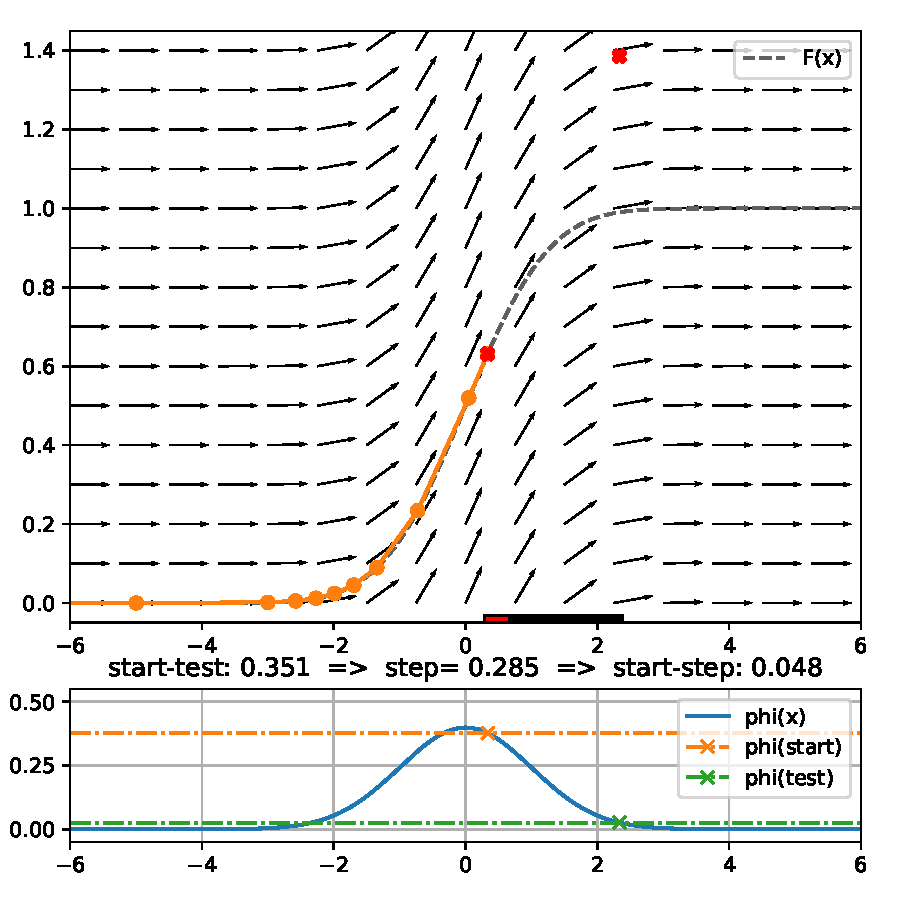
\includegraphics[width=0.75\textwidth]{papers/steps/img/ssc.pdf}
  \caption{Berechnung der Wahrscheinlichkeitsfunktion $F(x)$ der Standardnormalverteilung aus dessen Dichtefunktion
    (oben mit Pfeilen, unten als Funktion \texttt{phi(x))} mit einer einfachen Schrittweitensteuerung
    \label{buch:steps:examplessc}}
\end{figure}

\subsection{Schrittweitensteuerung nach Fehlberg
  \label{steps:subsection:fehlberg}}
\begin{figure}
  \centering
  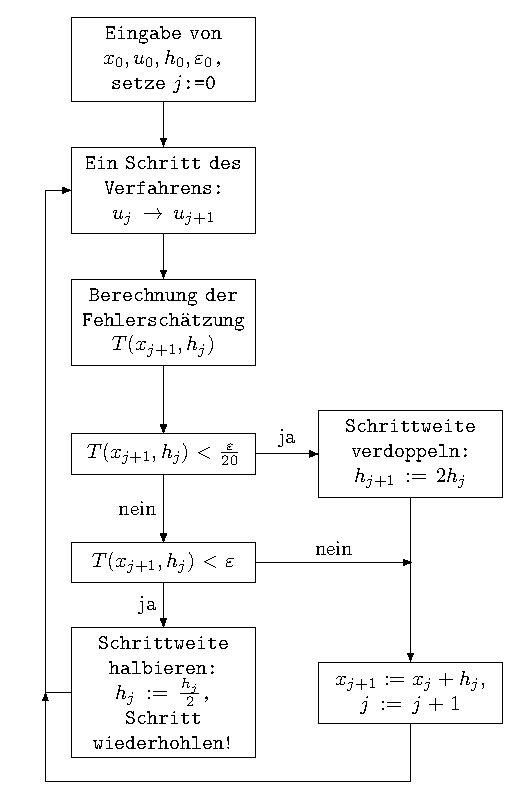
\includegraphics[width=0.5\textwidth]{papers/steps/img/Fehlberg_Flowchart.pdf}
  \caption{Algorithmus zur Schrittlängensteuerung mittels Fehlerschätzung nach Fehlberg
  \cite{steps:Numerische-Mathematik}
    \label{buch:steps:flowchartfehlberg}}
\end{figure}%
Ein anderer Ansatz zur Realisierung einer Schrittweitensteuerung ist mittels der Fehlerschätzung nach Fehlberg
\index{Fehlerschätzung}%
\index{Fehlberg}%
Dabei wird der Fehler des aktuellen Schrittes anhand der Differenz zweier unterschiedlicher, paralleler
Runge-Kutta Schritte geschätzt. Durch geschickte Kombination dieser beiden Schritte
lässt sich der Mehrrechenaufwand dazu aber merklich reduzieren, was in der Literatur als \textit{einbetten} bezeichnet wird.
\index{einbetten}%
\index{Einbettung}
Damit diese Einbettung möglich wird, sind die einzelnen Stufen etwas anders verteilt und gewichtet als im Abschnitt
\ref{subsection:buch:ode:runge-kutta}.
Wie solche Parameter für die einzelnen Stufen bestimmt werden können, wurde im Abschnitt
\ref{buch:subsection:quadratischeverfahren}
an Hand des verbesserten Euler-Verfahrens und des vereinfachten Runge-Kutta-Verfahrens
erläutert.
Weitere Details zum folgenden Beispiel sind im Kapitel \textit{Eingebette Verfahren und Schritteitensteuerung}
des Buchs
\cite{steps:Numerische-Mathematik}
zu finden.
In diesem Beispiel wird gezeigt, wie ein Runge-Kutta Schritt 4. Ordnung (5 Stufen) in ein Schritt 5. Ordnung (6 Stufen) eingebettet wird.
Dabei werden zuerst alle Koeffizienten berechnet, welche für den Schritt 4. Ordnung nötig sind:
\begin{align*}
  k_1 & =f(x_j, u_j),                                                                           \\
  k_2 & =f\left(x_j + \frac{2}{9}h, u_j+\frac{2}{9}hk_1\right),                                            \\
  k_3 & =f\left(x_j + \frac{1}{3}h, u_j+\frac{1}{12}hk_1+\frac{1}{4}hk_2\right),                           \\
  k_4 & =f\left(x_j + \frac{3}{4}h, u_j+\frac{69}{128}hk_1-\frac{243}{128}hk_2+\frac{135}{64}hk_3\right),  \\
  k_5 & =f\left(x_j + h, u_j-\frac{17}{12}hk_1+\frac{27}{4}hk_2-\frac{27}{5}hk_3+\frac{16}{15}hk_4\right).
\end{align*}
Daraus kann eine erste Schätzung für den Punkt am Schrittende gemacht werden:
\[
  u_{j+1} =u_j +h\cdot\left(\frac{1}{9}k_1+\frac{9}{20}k_3+\frac{16}{45}k_4+\frac{1}{12}k_5\right).
\]
Mit einem weiteren Koeffizienten
\[
  k_6 =f\left(x_j + \frac{5}{6}h, u_j+\frac{65}{432}hk_1-\frac{5}{16}hk_2+\frac{13}{16}hk_3+\frac{4}{27}hk_4+\frac{5}{144}hk_5\right)
\]
lässt sich nun eine zweite Schätzung für den Endpunkt berechnen:
\[
  \hat{u}_{j+1} =u_j+h\cdot\left(\frac{47}{450}hk_1+\frac{12}{25}hk_3+\frac{32}{225}hk_4+\frac{1}{30}hk_5+\frac{6}{25}hk_6\right).
\]
Der lokale Fehler des Schrittes lässt sich nun mit
\[
  T(x_{j+1},h)=|u_{j+1}-\hat{u}_{j+1}|=\frac{h}{300}\cdot|-2k_1+9k_3-64k_4-15k_5+72k_6|
\]
schätzen.
Da beide Schätzungen eine Linearkombination der Koeffizienten $k_1$ bis $k_6$ sind,
lässt sich die Differenz auch direkt aus den Linearkombinationen ermitteln,
sodass der zweite Schätzwert $\hat{u}_{j+1}$ überflüssig wird.

\begin{figure}
  \centering
  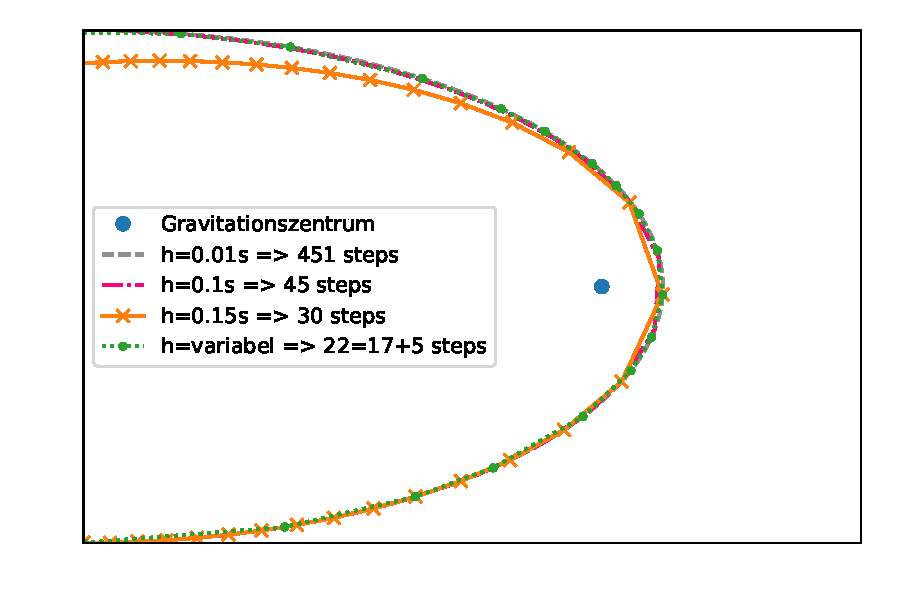
\includegraphics[width=\textwidth]{papers/steps/img/comparison_fehlberg_ssc.pdf}
  \caption{Bahn eines Teilchens um ein Gravitationszentrum: Vergleich von unterschiedlichen fixen Schrittweiten
  mit der variablen Schrittweite mittels Fehlerschätzung nach Fehlberg und Steueralgorithmus nach Abbildung~\ref{buch:steps:flowchartfehlberg},
  wiederholte Schritte beim Verkleinern der Schrittweite mitberücksichtigt}
  \label{buch:steps:comparisonFixedVariableFehlberg}
\end{figure}%

Mit dieser Fehlerschätzung lässt sich nun ein Algorithmus wie in Abbildung ~\ref{buch:steps:flowchartfehlberg} steuern,
welcher die Schrittlänge kontrolliert. Falls die Schätzung des Fehlers $T(x_{j+1}, h_j)$ grösser ist als die erlaubte Toleranz $\varepsilon$,
wird die Schrittweite halbiert und der Schritt wiederholt.
Falls der Fehler viel kleiner ist als die erlaubte Toleranz, wird die Schrittweite für den nächsten Schritt verdoppelt.
Im Beispiel in Abbildung~\ref{buch:steps:comparisonFixedVariableFehlberg} lässt sich somit die nötige Anzahl Schritte
im Vergleich zu einer ähnlich genauen, fixen Schrittweite etwa halbieren.


